\chapter{Results}

\section{Exploiting Android x86}

\begin{listing}[H]
  \singlespacing
  \inputminted[]{text}{source/crash-input}
  \caption{Crash Input}
  \label{lst:crash-input}
  \onehalfspacing
\end{listing}

Listing~\ref{lst:exploit-scenario1-progress} shows the progress of exploit
generation. A file, also known as ``crash input'', as shown in
Listing~\ref{lst:crash-input}, with 90 (0x5a) bytes of the size is mapped into
memory and marked as symbolic as shown on line 8. Starting from line 10, the
message indicates that some part of the symbolic data has tainted the EIP
register and thus triggers the exploit generating process. The record shows
that the EIP register is overwritten by value 0x61616161, which is the
hexadecimal representation of the string ``aaaa'', starting from the 27th
(0x1b) byte of the overall symbolic data.  The process then searches through
all memory space to collect memory chunks that are tainted by the symbolic
input. We name these chunks of memory as symbolic array. In this example, three
symbolic arrays all with size 90 bytes have been found. The process then tries
to inject three pieces of data into a symbolic array, a piece of pre-generated
shellcode, a NOP sled, and the address pointed to somewhere in-between the NOP
sled. The process would start to generate exploit with the largest array, and
move on to the next one if the current one does not satisfy all the
constraints.

\begin{listing}[H]
  \singlespacing
  \inputminted[fontsize=\footnotesize, linenos]{text}{source/exploit-scenario1-progress}
  \caption{Exploit Progress of Scenario 1}
  \label{lst:exploit-scenario1-progress}
  \onehalfspacing
\end{listing}

An example of generated exploits is shown as Listing~\ref{lst:exploit-input} in
hexadecimal format. The exploit input first starts with several `0x01' bytes.
These `0x01' are chosen by the solver, since there is no constraint related to
these bytes. Followed by are four bytes that will overwritten the EIP register,
``0x080e9075'' in little-endian order. The last part is the shellcode that will
write the string ``Exploit!'' into Android logging service. The shellcode could
be considered the same as the following C code snippet

\inputminted[fontsize=\footnotesize]{c}{source/execve-log.c}

\begin{listing}[H]
  \singlespacing
  \inputminted[]{text}{source/exploit-input-80e9075}
  \caption{Generated Exploit Input}
  \label{lst:exploit-input}
  \onehalfspacing
\end{listing}

\begin{figure}[!ht]
  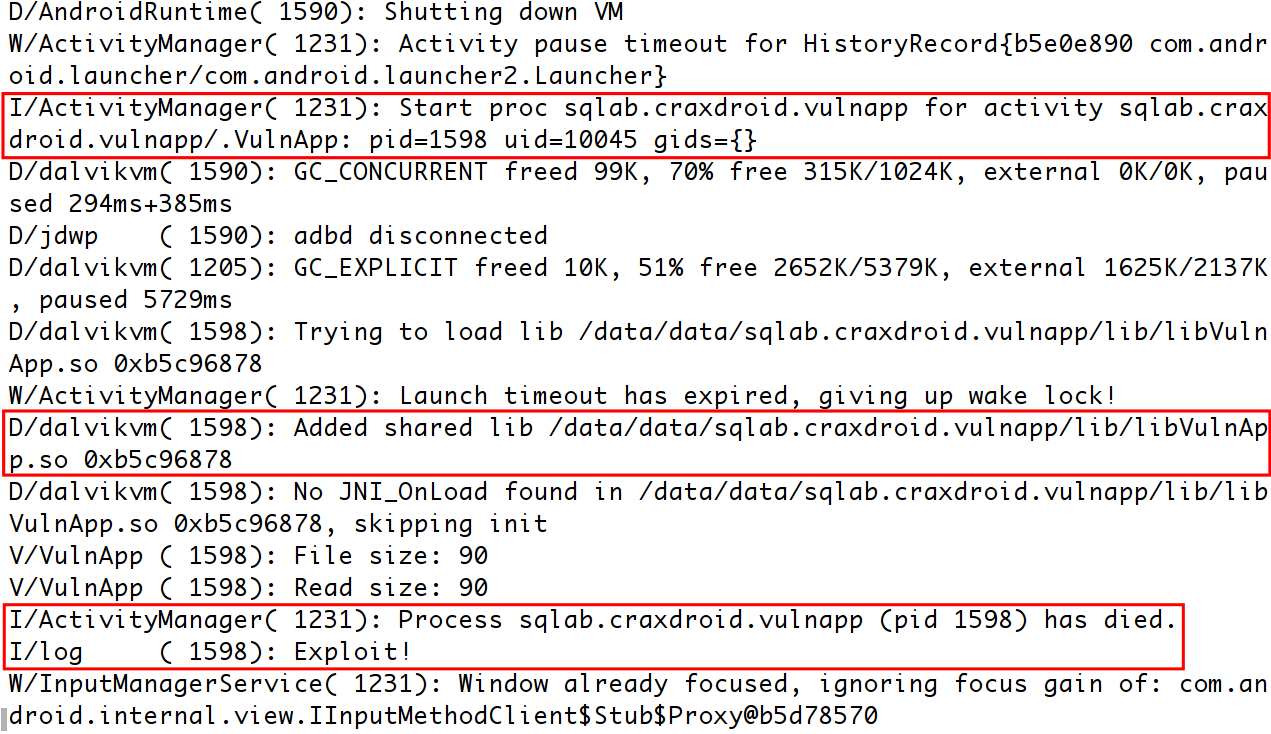
\includegraphics[width=\textwidth]{exploit-verify}
  \caption{Android x86 Exploit Verification}
  \label{fig:exploit-verify}
\end{figure}

Finally, the generated exploit file is fed back to the vulnerable app to verify
that it is a usable exploit. As shown in Figure~\ref{fig:exploit-verify}, the
vulnerable app is fired up and loads the native library correctly. The process
is then hijacked by our exploit. The ActivityManger figures out that the
process is dead, so it logs down the incident. And the following message---
``Exploit!'', indicates that the exploit succeeds.

\begin{listing}[H]
  \singlespacing
  \inputminted[fontsize=\footnotesize, linenos]{text}{source/exploit-scenario2-progress}
  \caption{Exploit Progress of Scenario 2}
  \label{lst:exploit-scenario2-progress}
  \onehalfspacing
\end{listing}
